
\section{Background and Motivating Example}
\subsection{System Monitoring}
System monitoring collects auditing events about the system calls that are crucial in security analysis, describing the interactions between system entities and resources.
As shown in previous studies~\cite{backtracking,backtracking2,taser,wormlog,gao2018saql,gao2018aiql,mcitracking,logtracking}, on main-stream operating systems (Windows, Linux, and Mac OS), system entities in most cases are files, network connections, and processes~\cite{backtracking,backtracking2,taser,wormlog},
and the collected system calls are mapped to three major types of system events:
(i) process creation and destruction, (ii) file access, and (iii) network access.
As such, we consider \emph{system entities} as \emph{files}, \emph{processes}, and \emph{network connections}.
We define an interaction among entities as an \emph{event}, which is represented using the triple \emph{$\langle$subject, operation, object$\rangle$}.
% We categorize events into three types according to the type of their object entities, namely \emph{file events}, \emph{process events}, and \emph{network connection events}.


\eat{
\begin{table}[!t]
	\centering
	\caption{Representative attributes of system entities.}\label{tab:entity-attributes}
	\begin{adjustbox}{width=0.48\textwidth}
		\begin{tabular}{|l|l|}
			\hline
			\textbf{Entity}		&\textbf{Attributes}\\\hline
			File				&PathName, etc.\\\hline
			Process			&PID, Name, User,  etc.\\\hline
			Network Connection	& IP, Port, Protocol \\\hline
		\end{tabular}
	\end{adjustbox}
	%	\vspace*{-2ex}

	\vspace*{1ex}
\end{table}
}


\begin{table}[t]
	\centering
	\caption{Representative attributes of system entities}
	\label{tab:entity-attributes}
	\resizebox{0.44\textwidth}{!}{%
		\begin{tabular}{l|l|l}
			\hline
			\textbf{Entity}             & \textbf{Attributes}    & \textbf{Shape in Graph} \\ \hline
			File               & Name, Path          & Ellipse        \\
			Process            & PID, Name, User, Cmd  & Square         \\
			Network Connection & IP, Port, Protocol   & Parallelogram  \\ \hline
		\end{tabular}%
	}
\end{table}


% \eat{
% \begin{table}[!t]
% 	\centering
% 	\caption{Representative attributes of system entities}\label{tab:entity-attributes}
% 	\begin{adjustbox}{0.45\textwidth}
% 		\begin{tabular}{|l|l|}
% 			\hline
% 			\textbf{Entity}		&\textbf{Attributes}\\\hline
% 			File				&Path\\\hline
% 			Process			&PID, Name, User, Cmd\\\hline
% 			Network Connection	& IP, Port, Protocol \\\hline
% 		\end{tabular}
% 	\end{adjustbox}
% 	%	\vspace*{-2ex}

% 	\vspace*{1ex}
% \end{table}
% }

\begin{table}[!t]
	\centering
	\caption{Representative attributes of system events.}\label{tab:event-attributes}
	\begin{adjustbox}{width=0.45\textwidth}
		\begin{tabular}{|l|l|}
			\hline
			\textbf{Operation}		& Read/Write, Execute, SendTo/Recvmsg\\\hline
			\textbf{Time}		& Start Time/End Time, Duration\\\hline
			\textbf{Misc.}		& Subject, Object, Failure Code\\\hline
		\end{tabular}
	\end{adjustbox}
	%	\vspace*{-2ex}

		\vspace*{1ex}
\end{table}

\begin{figure*}
    \centering
    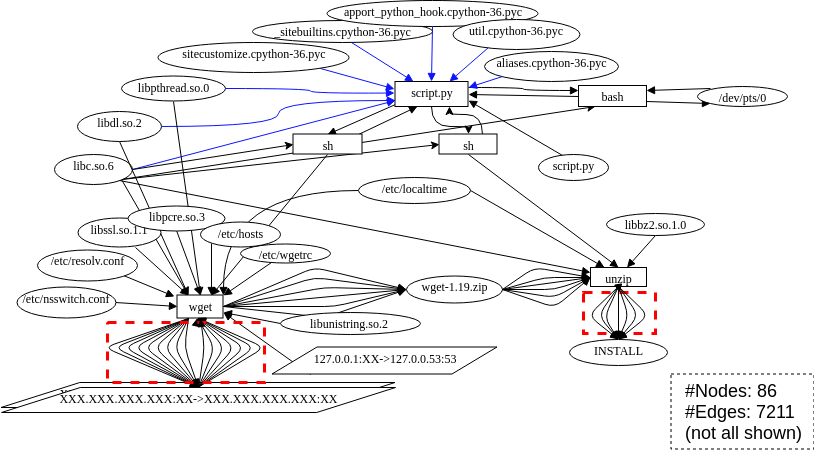
\includegraphics[width=0.8\textwidth]{figs/fig-before.png}
    \caption{Simplified dependency graph for downloading a zip file and performing decompression}
    \label{fig:before}
\end{figure*}

Entities and events have various attributes (\cref{tab:SystemEntity,tab:event-attributes}).
The attributes of an entity include the properties to describe the entities (\eg file name, process name, and IP address),
and the unique identifiers to distinguish entities (\eg file path and process ID).
The attributes of an event include event origins (\ie start time/end time),
operations (\eg file read/write),
and other security-related properties (\eg system call return code).




\subsection{Causality Analysis}
Causality analysis analyzes the auditing events to infer the dependencies among system entities and present the dependencies as a directed graph.
In the dependency graph $G(E,V)$, a node $v \in V$ represents a process, file or network socket.
An edge $e = (u, v) \in E$ indicates a system auditing event involving two entities $u$ and $v$ (\eg process creation, file read or write, and network access), and its direction (from the source node $u$ to the sink node $v$) indicates the data flow.
Each edge is associated with a time window, $tw(e)$.
We use $ts(e)$ and $te(e)$ to represent the starting time and the ending time of $e$.
Formally, in the dependency graph, for two event edges $e_1 = (u_1, v_1) $ and $e_2 = (u_2, v_2)$, there exist causality dependency between $e_1$ and $e_2$ if $v_1 = u_2$ and $ts(e_1) < te(e_2)$.

Causality analysis enables two important security applications:
(i) \emph{backward causality analysis} and (ii) \emph{forward causality analysis}.
Given a POI event $e_s(u,v)$, a backward causality analysis traces back from the source node $u$ to find all events that have causality dependencies on $u$,
and a forward causality analysis finds all events on which $v$ have causality dependencies.
Backward causality analysis can help identify the entry points of attacks 
and forward causality analysis can help investigate the ramification of attacks.


\subsection{Motivating Example}
\cref{fig:before} shows an example dependency graph for a representative system task:
a process \incode{script.py} executes \incode{wget} to download a file named \incode{wget-1.19.zip}, and unzips it to obtain the file \incode{INSTALL}.
Such task is often seen in malicious payloads~\cite{securitybook}.
The POI event of the graph is the event that creates the file \incode{INSTALL}.
The original dependency graph obtained by applying causality analysis on the POI event contains 86 nodes and 7211 edges.
Due to space limit, only relevant part is shown in the figure.

\begin{figure}
    \centering
    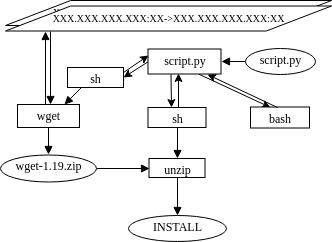
\includegraphics[width=0.4\textwidth]{figs/fig-after.png}
    \caption{The critical edges of the dependency graph in Fig.~\ref{fig:before}}
    \label{fig:after}
\end{figure}

\myparatight{Surfacing Critical Edges}
The first goal of attack investigation using dependency graph is to surface attack provenance, \ie finding critical edges.
\cref{fig:after} shows the 14 critical edges of the example dependency graph.
Obviously, it requires non-trivial efforts to search these critical edges from the huge dependency graph with 86 nodes and 7211 edges, and there is a strong need to automate this identification process.

However, causality analysis~\cite{backtracking,backtracking2} typically uses time windows to make decisions on whether an edge has causal dependency on the POI event, which contains limited information to distinguish critical edges.
For example, the \incode{script.py} process node has many incoming edges, but the edges marked in blue are coming from system libraries, which give little information on surfacing the attack provenance, while the edges that connect to the process \incode{sh} show much more useful information for investigating the task.
But all these edges cannot be pruned since the end times of their time windows are all before the POI event. 

To address this challenge, \tool leverages the insight that critical edges often possess properties that are different from non-critical edges: (i) the time difference between the critical edges and the POI event is usually small;
(ii) the data amount processed by the critical edges is similar to the target file in the POI event;
(iii) source nodes of non-critical edges have either no incoming edges (\eg system libraries) or many outgoing edges (\eg long-running processes), while the source node of the critical edges usually has only a few incoming edges and only a few outgoing edges (\ie ``high concentration'').
To capture these properties, \tool computes three novel features for each edge: \emph{relative time difference}, \emph{relative data amount difference}, and \emph{concentration degree} (details in \cref{sec:approach}), and use them to determine the weight for each edge, producing a weighted dependency graph.

Note that with the weights on the edges, security analysts can control the threshold value on hiding some non-critical edges with low weights when identifying the critical edges.
But when the security analysts need to look into some part of the graph with more details,
he may lower the threshold value and the non-critical edges that contain more detailed information (\eg library files) will be shown.

\myparatight{Reputation Propagation}
The second goal of attack investigation using dependency graph is to determine whether the file \incode{INSTALL} contains malicious payloads. 
If we look at the critical edges, we can trace back from \incode{INSTALL} to \incode{script.py}, which is the creator of \incode{INSTALL}.
This indicates that if \incode{script.py} is suspicious, \incode{INSTALL} is very likely to contain malicious payloads; otherwise, \incode{INSTALL} is likely to be a benign installation script.

To automate the process in inspecting the dependency graph for determining whether a POI event contains malicious payloads, \tool performs reputation propagation on the weighted dependency graph.
In this example, if we assume \incode{script.py} is suspicious (\ie $0$), and all the system libraries with a neural reputation (\ie 0.5).
Then \tool propagates the reputation from these seed nodes through all the edges, where the weights of the edges are proportional to the reputation being propagated from the nodes.
Thus, if the weights of the critical edges are significantly higher than the weights of the non-critical edges, the contribution from \incode{script.py} to \incode{wget} dominates the contributions from system libraries to \incode{wget}.
This will cause \incode{INSTALL} to have a reputation close to 0, which is similar to \incode{script.py}, but not the system libraries.
In this way, \tool can automatically determine that \incode{INSTALL} is very likely to contain malicious payloads.







\eat{
It only shows the relevant part about this task. \eat{The original causal graph of the host contains $154$ nodes and $7958$ edges. Although we already filter out all the irrelevant system entities, it still contains $86$ nodes and $7211$ edges. that represents system packages and duplicate edges.} The edge in the red square shows several file write and network communication events. The blue edge represents the system packages' effect on the state of process.




\pfang{original node: }
One typical challenge is that the dependency graph is too large to analyze, with thousands even million of edges. Given such a large number of edges, the critical edges are buried. Figure ~\ref{fig:before} is a typical download and decompress process. We extract relevant parts from the original graph, it contains 154 nodes and 7958 edges. For the dependency graph only about this download process, it still contains 86 nodes and 7211 edges. To find a critical path showed in Fig.~\ref{fig:after} about this process among 7211 edges is a daunting task. \textcolor{red}{sounds like this part end with no conclusion. We may briefly say how we will address this problem and refer to teh corresponding section.}





such as 
Given events $evt_1$ and $evt_2$, to construct a backward (forward) dependency $evt_1$ $\xrightarrow{backward}$ $evt_2$ ($evt_1$ $\xrightarrow{forward}$ $evt_2$), $evt_1$ must occur after (before) $evt_2$. Causality analysis can be used to analyze the \emph{causality} of an anomalous event, such as the creation of an unknown executable in a system. Assume that we identified a malicious script in the web server, to understand how it infects a victim machine, we can start the investigation of the process that executed or read from the script,
and trace whether they propagate the malicious scripts across hosts.

In this project, the goal of this step is to reconstruct the time line in an attack. First, we need a formal definition of important terms and concepts used in our method.
First, two events have \textit{causality dependency} with each other if an event has information flow that affect the other event.\\
DEFINITION 1: \textbf{Causality Dependency} \\
\indent For two event edges $e_1 = \mathit{(u_1, v_1)} $ and $e_2 = \mathit{(u_2, v_2)} $ , they have causality dependency, if
\begin{itemize}[noitemsep]
	\item $v_1 = u_2 $
	\item $te\mathit{(e_1)} < te\mathit{(e_2)}$
\end{itemize}
if $e_1$ has information flow to $e_2$ and $e_2$ has information flow to $e_3$, then $e_1$ and $e_3$ have causality dependency. In the graph, a dependency relationship is represented as an edge, the edge direction is same as the direction of of information flow that is decided by the system event. To be more specific, if a process calls Linux system event "read" to read data from config files, the source of the edge is the file and the target is the process.
}


